% !TEX root = ../../../main.tex
% 来源：中学数学实验教材·第二册（几何）
% 章节：实验几何 / 方向、角度与平行
% 原始文件：1.tex，行 929-940
% 类型：tikz
% ---
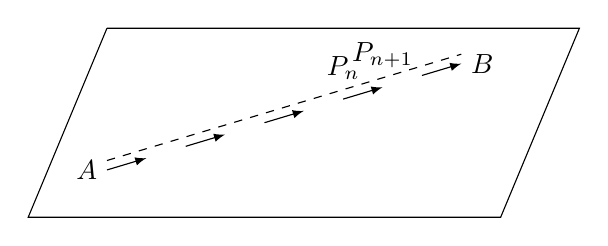
\begin{tikzpicture}[>=latex, yscale=.6]
	\draw(1,4)--(7,4)--(6,0)--(0,0)--(1,4);
	\draw[->](1,1)node[left]{$A$}--(1.5,1.25);
	\draw[->](2,1.5)--(2.5,1.75);
	\draw[->](3,2)--(3.5,2.25);
	\draw[->](4,2.5)--(4.5,2.75);
	\draw[->](5,3)--(5.5,3.25)node[right]{$B$};
	\draw[dashed](1,1.2)--(5.5,3.45);
\node at (4,2.7)[above]{$P_n$};
\node at (4.5,2.95)[above]{$P_{n+1}$};

\end{tikzpicture}
